\chapter{Performant Web Applications}%
\label{cha:performant_web_applications}

\minitoc%

\section{A Brief History of Native Code in the Client}%
\label{sec:native_client}

Being able to run high performance code in the browser
unlocks many use cases, including scientific computing.
Yet, it remains a challenging task.
Resources often refers to this as ``native'' code
but the terminology is rather vague.
Depending on the context, it may have one of the following meanings,
\begin{enumerate}
\setlength\itemsep{-0.5em}
	\item code statically compiled directly to the target architecture and running from the browser,
	\item code compiled from a typical ``native'' language such as C or C++,
	\item or anything that is not generating JavaScript.
\end{enumerate}
The distinction between those and how they relate to ``native'' code
will be made clearer after a brief history of high performance code in browsers.

\subsection{Java Applets}%
\label{sub:java_applets}

In 1995, just four years after the birth of the Web,
the Java programming language was created.
It appeared with a companion technology called Java Applet,
designed to run Java applications in the browser.
The Java Virtual Machine (JVM) was hosted by browsers,
enabling much better performances than JavaScript at that time.
As an example, Brendon C. Glazer worked on interactive ray tracing
of VRML scenes with Java applets in 1999~\cite{Glazer1999InteractiveRT}.
Figure~\ref{fig:glazer-thesis} depicts how the applet would appear
in a Web page at that time.
Since 1998 Java applets have also had access to 3D hardware acceleration~\cite{Java3dAPISpec}
whereas JavaScript waited until 2011 for WebGL in HTML5 canvas.

\begin{figure}[h!]
	\centering
	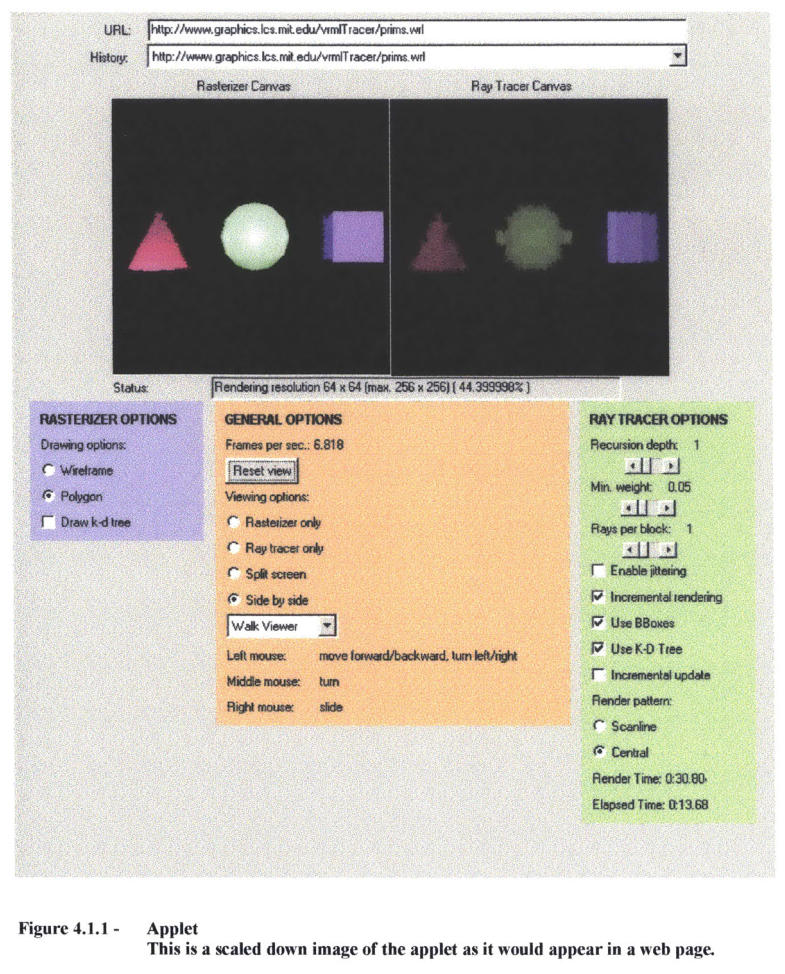
\includegraphics[width=\linewidth]{assets/img/glazer-thesis.jpg}
	\caption{Interactive ray tracing applet from Brendon C. Glazer master thesis (1999).}%
	\label{fig:glazer-thesis}
\end{figure}

On the down side, Java applets would break accessibility of the Web.
Screen readers would not be able to parse the content of the dedicated
applet area in the page.
The security model of Java applets was also quite risky.
Applets would have to get approved by a browser user and then gain rights
equivalent to a native application on your desktop.
Unfortunately, just like terms of service, most people just click ``agree''
and move on.
In addition, the Java Runtime Environment (JRE) has had hundreds of security
vulnerabilities~\cite{JreCve} in its lifetime.
This represents a serious security threat for browser vendors.
Java applets were eventually entirely removed from Java SE 11, in 2018.

\subsection{Flash}%
\label{sub:Flash}

In his ``History of Flash''~\cite{HistoryFlash}, Jonathan Gay retraces the early days of Flash.
In 1993, he, Charlie Jackson and Michelle Welsh founded FutureWave Software
but their initial vector drawing application did not draw much attention (pun intended).
After discussions at Siggraph 1995, the company decided to focus on a web animation
product named ``FutureSplash Animator''.
It gained reputation with Microsoft and Disney using it and as a consequence,
was acquired by Macromedia and rebranded ``Flash'' in 1996.

Contrary to Java applets, Flash use cases started very narrow.
It provided a simple and efficient solution to build and share animations on the web,
giving a visual advantage over pure HTML documents.
In year 2000, Flash 5 was released, with the ActionScript programming language,
bringing even more potential to Flash-based websites.
Two years later, in 2002, Flash 6 brought support for real-time messaging protocols,
enabling video and audio streaming capabilities.
This represents roughly 8 years until 2010 when such capabilities are also
supported through HTML5 in most browsers.
In the meantime, highly influencial projects shaped the Web thanks to Flash.
You may have heard of Chad Hurley, Steve Chen and Jawed Karim who launched
YouTube in 2005, based on Flash.

In spite of the many advantages of Flash and ActionScript over classic Web pages,
it also had similar flaws than Java applets.
In October 2000, usability consultant Jakob Nielsen published a short article
entitled ``Flash: 99\% Bad''~\cite{FlashBadNielsen} stating that
``Flash technology tends to discourage usability for three reasons:
it makes bad design more likely,
it breaks with the Web's fundamental interaction style,
and it consumes resources that would be better spent enhancing a site's core value.''
Apple also played a huge role in Flash decline.
In 2007 the iPhone launched without Flash support,
leading to Steve Jobs, then Apple CEO, writing in 2010 an oppen letter called
``Thoughts on Flash''~\cite{FlashJobs}
in which he explains why Flash was doomed to disappear.
Among those reasons, Flash is proprietary, going against open Web standards,
it has numerous security flaws~\cite{FlashCVE}, and is the number one reason Macs crash.

Consequently, with the advent of HTML5 surrounding technologies regarding multimedia capabilities,
and the improved performances of JavaScript, Flash became obsolete.
So in July 2017, Adobe announced end support of Flash in 2020.

\subsection{Google Native Client (NaCl)}%
\label{sub:nacl}

Java applets and Flash were never trully considered ``native''
since they involved third party virtual machines.
You would not compile your code directly to machine instructions
but to an intermediate bytecode representation for Java applets,
or just using a JIT compiler for ActionScript (Flash) code.
They provided however great performances improvements when compared
to JavaScript before 2008 and the arrival of JavaScript JIT compilers with the V8 engine.
But around 2009 and 2010, two new projects named Native Client (NaCl) and Emscripten
respectively emerged from research at Google and Mozilla.
We will hold on Emscripten for now and explain first what NaCl was about.

At this period of time, native code was already running in browsers,
usually via an old plugin interface called the ``Netscape Plugin API'' (NPAPI).
This is how the JVM, the Flash player or PDF readers for example
would be integrated in browsers.
So from the observation that the Web had trully become a rich multimedia platform,
and that native code was already running in browsers via plugins,
a team of Google engineers explored a way to generalize and improve security
of any native C or C++ code execution in browsers~\cite{yee2009native}.
This would in theory unlock high performances for any Web application.
But it would need a sandboxed and secure new set of APIs
to make sure that those applications would not execute any malicious code via the browser.
That is how the Native Client (NaCl) project,
and its associated API called Pepper Plugin API (PPAPI) started in 2009.
I'll make the assumption that you got the NaCl and pepper joke \ldots

The two main downsides of this approach are the security and portability concerns.
Even though NaCl code would run into a sandboxed environment,
enforcing both security and accessibility to classical desktop resources
requires a continuous effort from browser vendors,
now needing to secure two different sandboxed environment,
NaCl and JavaScript, instead of one.
Portability was also a concern since any NaCl code would need to be compiled
to all target architectures where the browser need to run.
In practice, only x86 intel architectures were fully supported,
going against the nature of the Web, supposed to run on all platforms.
This limitation was the reason for the birth of the Portable Native Client project.

Portable Native Client (PNaCl, pronounced like the word ``pinnacle'', you get this one?),
was a work by A. Donovan et al.~\cite{donovan2010pnacl} aiming at distributing
NaCl programs in an intermediate pre-compiled neutral instruction-set format,
preventing the need to compile directly to all target architectures.
Concretely, the format chosen was the Low-Level Virtual Machine (LLVM) bitcode.
Unfortunately, this intermediate representation bitcode is a fast moving target,
and retrocompatibility is not a main objective of the LLVM project.
It means that PNaCl code could become obsolete at a fast pace,
also a deal breaker for Web standards.
With the reluctance of other vendors to adopt a non-specified Google initiative,
and the appeal of another rising approach coming from Emscripten,
PNaCl was finally deprecated in 2017.

\subsection{Emscripten and asm.js}%
\label{sub:emscripten-asmjs}

Out of curiosity, Mozilla engineer Alon Zakai started to work around 2010
on a project to explore the limitations of compiling C++ code to JavaScript.
It was the start of the Emscripten project~\cite{zakai2011emscripten}.
Emscripten base idea consists in converting LLVM bitcode to JavaScript.
LLVM originated from the work of
Chris Lattner and Vikram Adve~\cite{lattner2004llvm} on a compiler framework
and an intermediate code representation, optimized for compiler transformations.
It reduces the language-architecture complexity from $\mathcal{O}(mn)$ to $\mathcal{O}(m+n)$
since languages do not need to compile to every target like x86 or Arm,
and instead can just target LLVM which in turn knows how to compile to each
instruction set architecture (ISA) as depicted in Figure~\ref{fig:llvm}.

\begin{figure}[h]
	\centering
	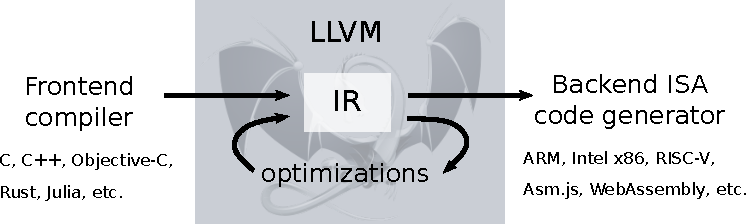
\includegraphics[width=\linewidth]{assets/img/llvm.pdf}
	\caption{LLVM Compiler Infrastructure}%
	\label{fig:llvm}
\end{figure}

After few iterations with the help of Luke Wagner, working on JavaScript compilation at Mozilla,
Emscripten was able to output JavaScript code running at roughly 2x to 4x native speed.
This specific subset of JavaScript was formalized under the name asm.js in 2013~\cite{herman2013asm}.
The asm.js code for a sum function is presented in Listing~\ref{lst:add-asmjs}.
As you can see, it makes use of JavaScript operations doing nothing,
like the bitwise-or with 0, except cohercing values to certain types.
You would not want to write asm.js code by hand, but for a compiler,
it enables certain kinds of optimizations not possible with traditional
hand-written JavaScript code.
Yet it is a strict subset of JavaScript and can still run in any browser,
whether or not they have a specialized handling of asm.js.

\lstinputlisting[%
	language=JavaScript,
	caption={Sum of two 32-bit integers in asm.js.},
	label={lst:add-asmjs}
]{assets/code/add-asm.js}

The performances without the need of any plugin convinced companies with huge
code bases to join the effort.
The Unreal game engine was ported, Autodesk AutoCAD~\cite{autocadweb}, Adobe Lightroom,
Facebook image compressions uploading code, OpenCV~\cite{taheri2018opencv} and many others.
With the success of Emscripten and asm.js as a proof of concept,
all major browser vendors came together to formalize a new specification
known today as WebAssembly.
Figure~\ref{fig:wasm-timeline} summarizes main events leading to the creation of WebAssembly.

\begin{figure}[h]
	\centering
	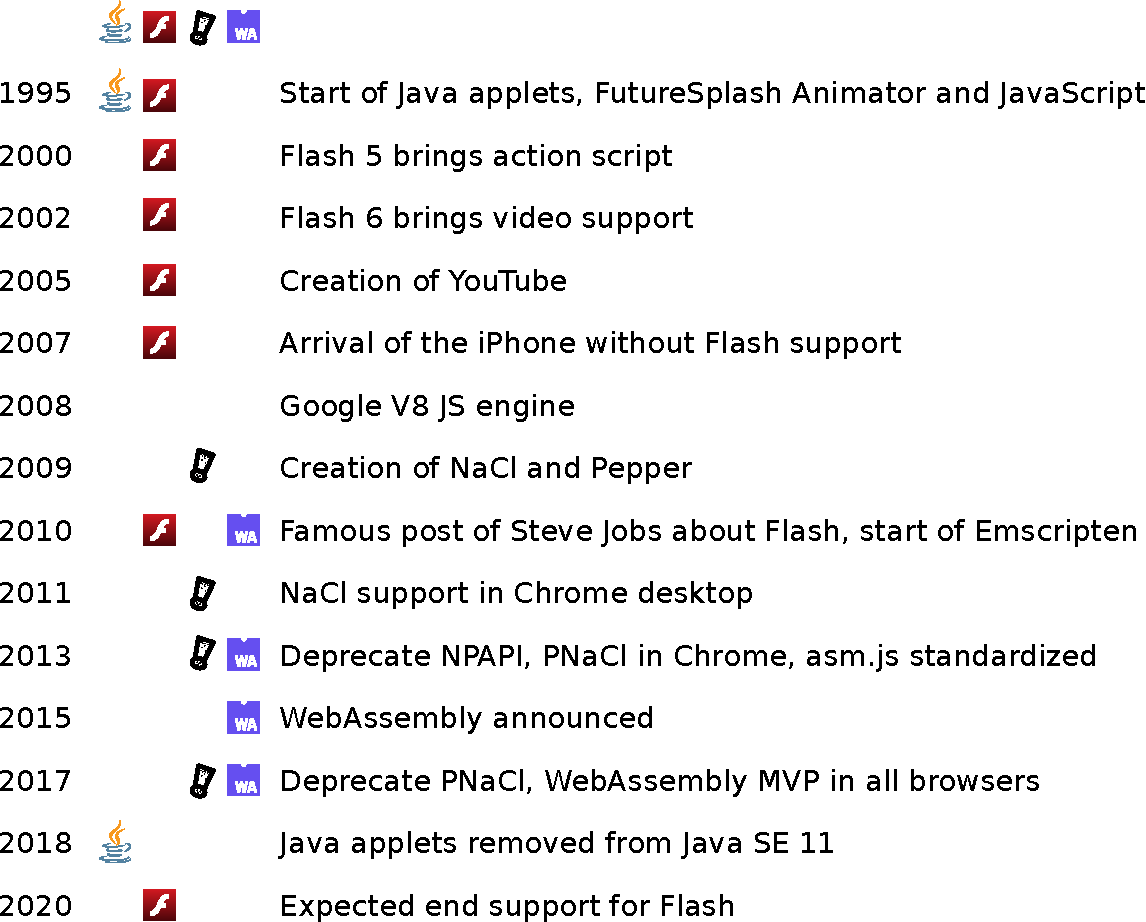
\includegraphics[width=\linewidth]{assets/img/wasm-timeline.pdf}
	\caption{Events releated to the birth of WebAssembly.}%
	\label{fig:wasm-timeline}
\end{figure}

\section{WebAssembly}%
\label{sec:WebAssembly}

WebAssembly, abreviated Wasm, is an instruction set with a binary format,
and a stack-based virtual machine able to execute those programs~\cite{haas2017bringing}.

\subsection{Relation to Previous Technologies}%
\label{sub:wasm_previous}

Just like Flash and Java applets, WebAssembly,
is executed by a virtual machine.
Similarly to NaCl, the Wasm runtime is sandboxed,
preventing it from accessing data outside of its context.
And as asm.js, Wasm does not require any plugin.
It has been developed as a Web standard and implemented
by all major Web browsers, desktop and mobile, since 2017.
Unlike asm.js however, Wasm is distributed in a binary format,
meaning it is more efficient to send over the network and to parse,
drastically reducing the loading time of Web pages.
WebAssembly has been built drawing lessons from the past and is going to endure
for the following reasons.

\begin{itemize}
	\item It is a Web standard and a collective effort from all browser vendors.
	\item It is the low level missing piece of the Web,
		complementing JavaScript where more control over performances is needed.
	\item It has strong security guaranties, and a sound type system~\cite{watt2018mechanising}.
	\item It theoretically enables any programming language to run on the Web.
\end{itemize}

\subsection{WebAssembly Minimum Viable Product (MVP)}%
\label{sub:wasm-mvp}

\subsection{WebAssembly Bright Future}%
\label{sub:wasm-future}

wasi, wapm, wasmer, interface types

WebAssembly: A New Compilation Target for the Web - Luke Wagner, April 12, 2016: https://youtu.be/89WPNeLnEyA
WebAssembly: Under the hood with Mozilla, March 7, 2017: https://youtu.be/o52\_5qAJhNg

\section{C++ portability pitfalls}%
\label{sec:cpp_pitfalls}

Code source (C++) -> LLVM IR -> Emscripten -> WebAssembly

Donc Emscripten a besoin du bitcode LLVM pour pouvoir compiler une base de code C++. En particulier, il n’est pas possible d’utiliser les bibliothèques précompilées (les “.so”) fournies par les OS dans les packages (apt-get install ...) dans ses dépendances. Toute dépendance (et ce récursivement) doit être recompilée avec Emscripten depuis le code source, et liée statiquement à la compilation de notre propre code. Par défaut, pour faciliter la vie, Emscripten intègre déjà la majorité de la librairie standard (std), et de certaines autres bibliothèques (SDL pour les applis graphiques, ...).

Example with image reading in OpenCV.
Had to rewrite PNG decoder.


DVO par exemple a des dépendances à OpenCV, Eigen, Boost, et Sophus. J’ai donc commencé par voir si j’arrive à compiler un programme minimaliste OpenCV avec Emscripten. Tout de suite les ennuis ont démarré. Au début, je n’ai même pas réussi à utiliser le build wasm de OpenCV (cf question sur stackoverflow). Je m’en suis finalement sorti, pour bloquer sur l’étape d’après, lire une image (cf question sur le forum OpenCV). En effet, dans la version wasm de OpenCV, la fonction imread a été remplacée par une méthode purement JavaScript qui prend un canvas en paramètre, et va donc directement récupérer la matrice depuis le canvas sans faire le décodage. Je pense que cette stratégie a été utilisée parce qu’en interne, la fonction imread OpenCV utilise la fonction imdecode, qui elle-même fait appel à une douzaine d’autres bibliothèques (libjpeg, libtiff, libpng, ...). J’ai essayé d’ajouter moi-même le module contenant la fonction imdecode au build wasm d’OpenCV mais je n’ai pas réussi à compiler ce module. J’ai tout un tas d’erreurs de "missing symbol" etc.

Ce n’est pas entièrement sans espoir, il faut le savoir ! Notamment, je n’ai besoin que du décodage png. Et libpng fait partie de ces quelques lib déjà intégrées à emscripten. En théorie je pourrais donc remplacer le code de décodage (cv::imdecode) par l’utilisation de libpng directement. Un des soucis c’est que l’API de libpng est super difficile à comprendre pour moi. Mais en théorie, le reste d’OpenCV qui est utilisé dans DVO fait partie du sous-ensemble qui devrait marcher.

Par contre, je n’ai pas fait de tests minimalistes avec les autres dépendances de DVO (eigen, boost, sophus) donc rien ne dit qu’on serait au bout de nos ennuis.

\section{Rust and WebAssembly}%
\label{sec:rust_wasm}

\begin{itemize}
	\item Rust programming language
	\item Wasm-bindgen
\end{itemize}
